%%%%%%%%%%%%%%%%%%%%%%%%%%%%%%%%%%%%%%%%%%%%%%%%%%%%%
%			      Video Out module					%
%					-----------						%
% Author: Thibault Porteboeuf						%
%%%%%%%%%%%%%%%%%%%%%%%%%%%%%%%%%%%%%%%%%%%%%%%%%%%%%

\section{VideoOut module}

\begin{figure}[H]
\center
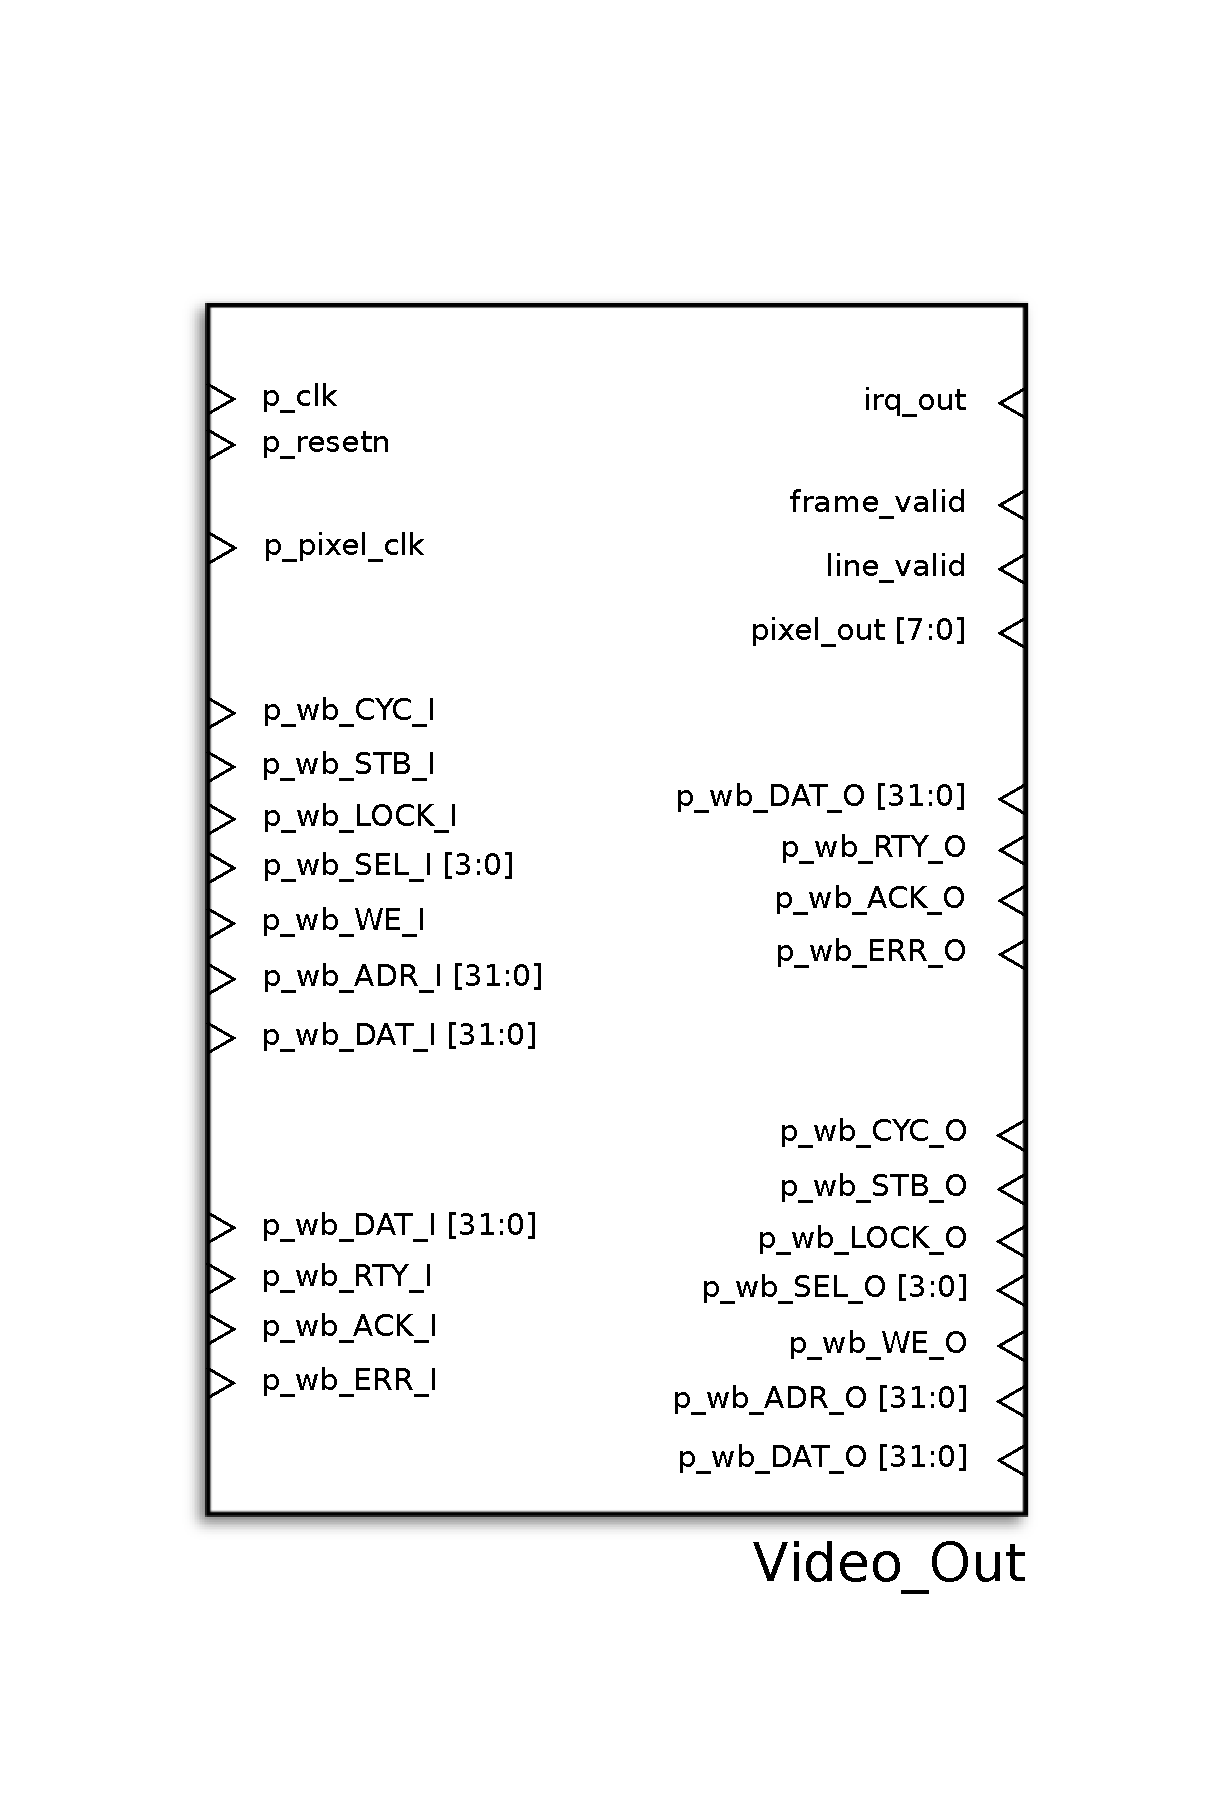
\includegraphics[width=7cm]{figs/Video_out.pdf}
\caption{VideoOut module's interface}
\label{VideoOut_interface}
\end{figure}

The VideoOut module is somewhat similar to the VideoIn module, as presented in figure \ref{VideoOut_struct}. They both include a one register slave module presented in section \ref{wb_reg_slave}, a wishbone master interface, and a state machine.


The main difference being that VideoOut generates the video signals as an output while reading from the RAM, whereas VideoIn handles the video signals as an input while writing to the RAM.

The different ports are detailed in figure \ref{VideoOut_interface}.

The module's behavior is described in the figure \ref{VideoOut_behavior}, and is enumerated as follows:
\begin{enumerate}
\item VideoOut remains Idle until an address to read to has been written to its slave interface
\item When this first configuration has been set, VideoOut starts preloading its internal buffer
\item VideoOut starts generating the video signals and poping pixels from the internal buffer
\item Each time the buffer is half empty, a read request is send over the wishbone bus by VideoOut's master interface, in order to retreive more data
\item This process continues until the end of the frame, which pauses the module. It then raises an Irq in order to get the next address to read to, and start over.
\end{enumerate}

Here again, the one register slave module is responsible for driving the Irq wire.
The state machines asks for an Irq to be raised, and the slave automatically acknowledges it once a write request has been received from the bus.

\vfill
\begin{figure}[h]
\center
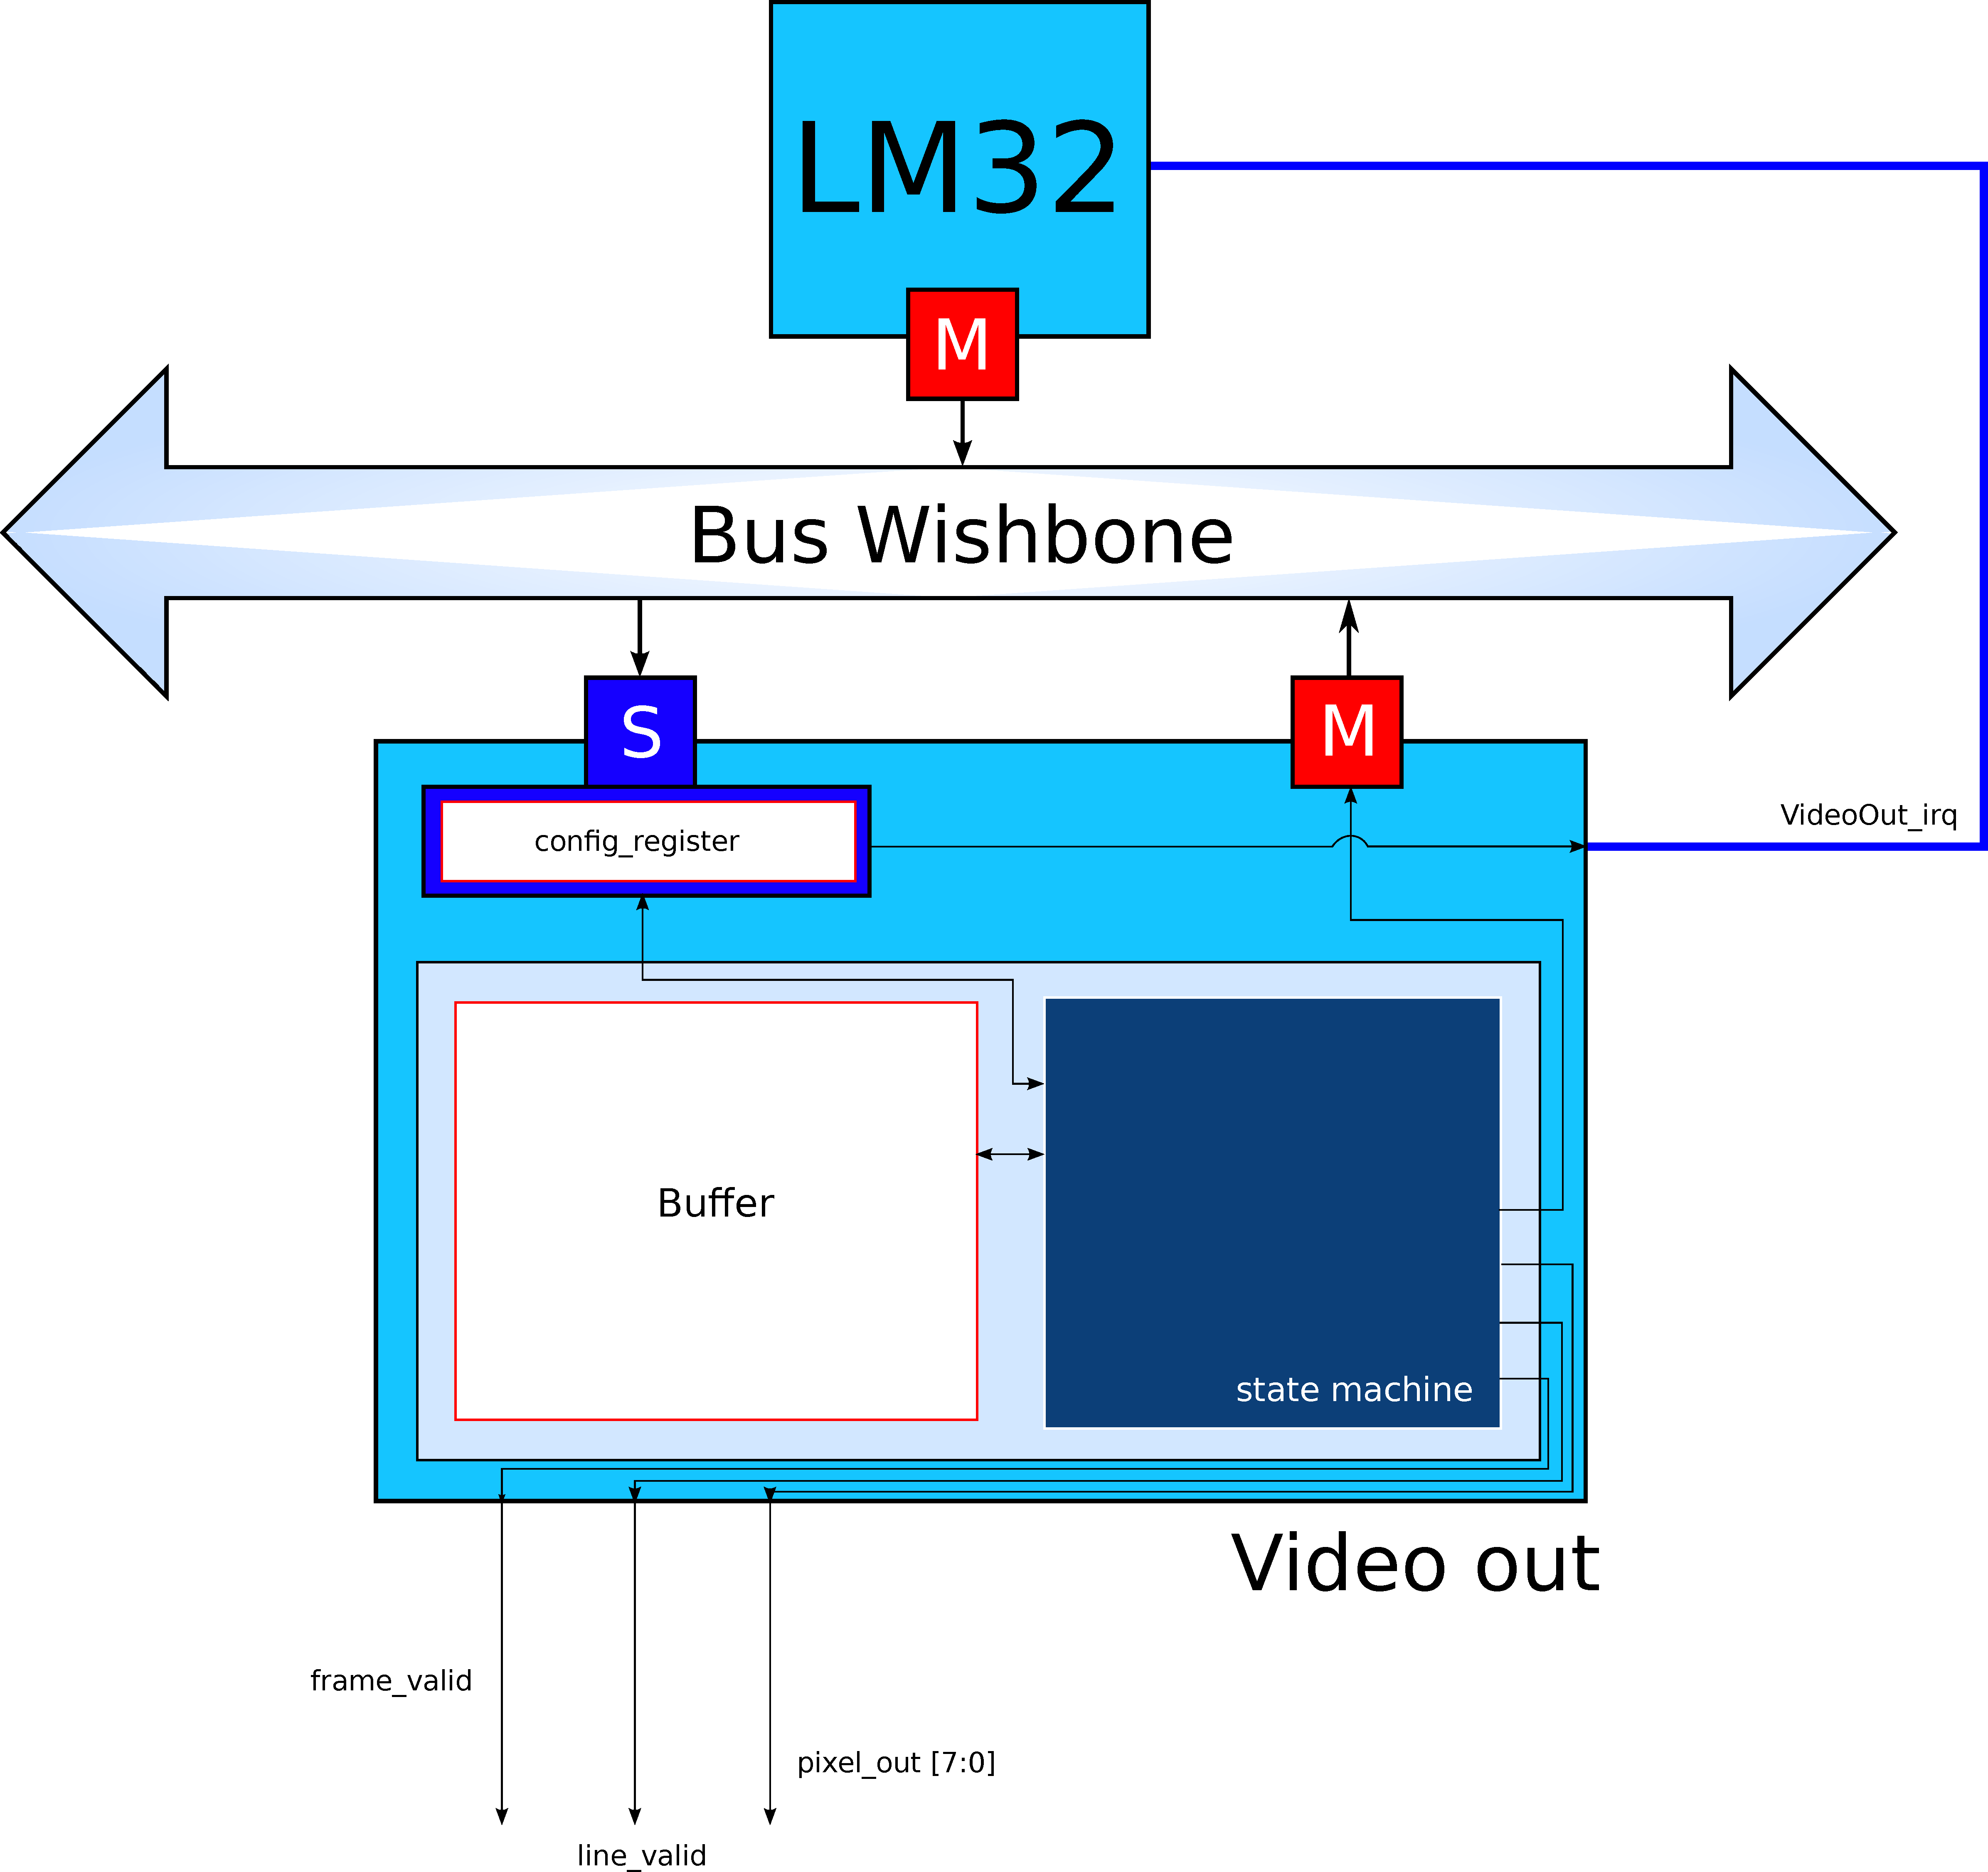
\includegraphics[width=11cm]{figs/Video_Out_blocks.pdf}
\caption{VideoOut's inner structure}
\label{VideoOut_struct}
\end{figure}
\vfill

\begin{figure}[h]
\center
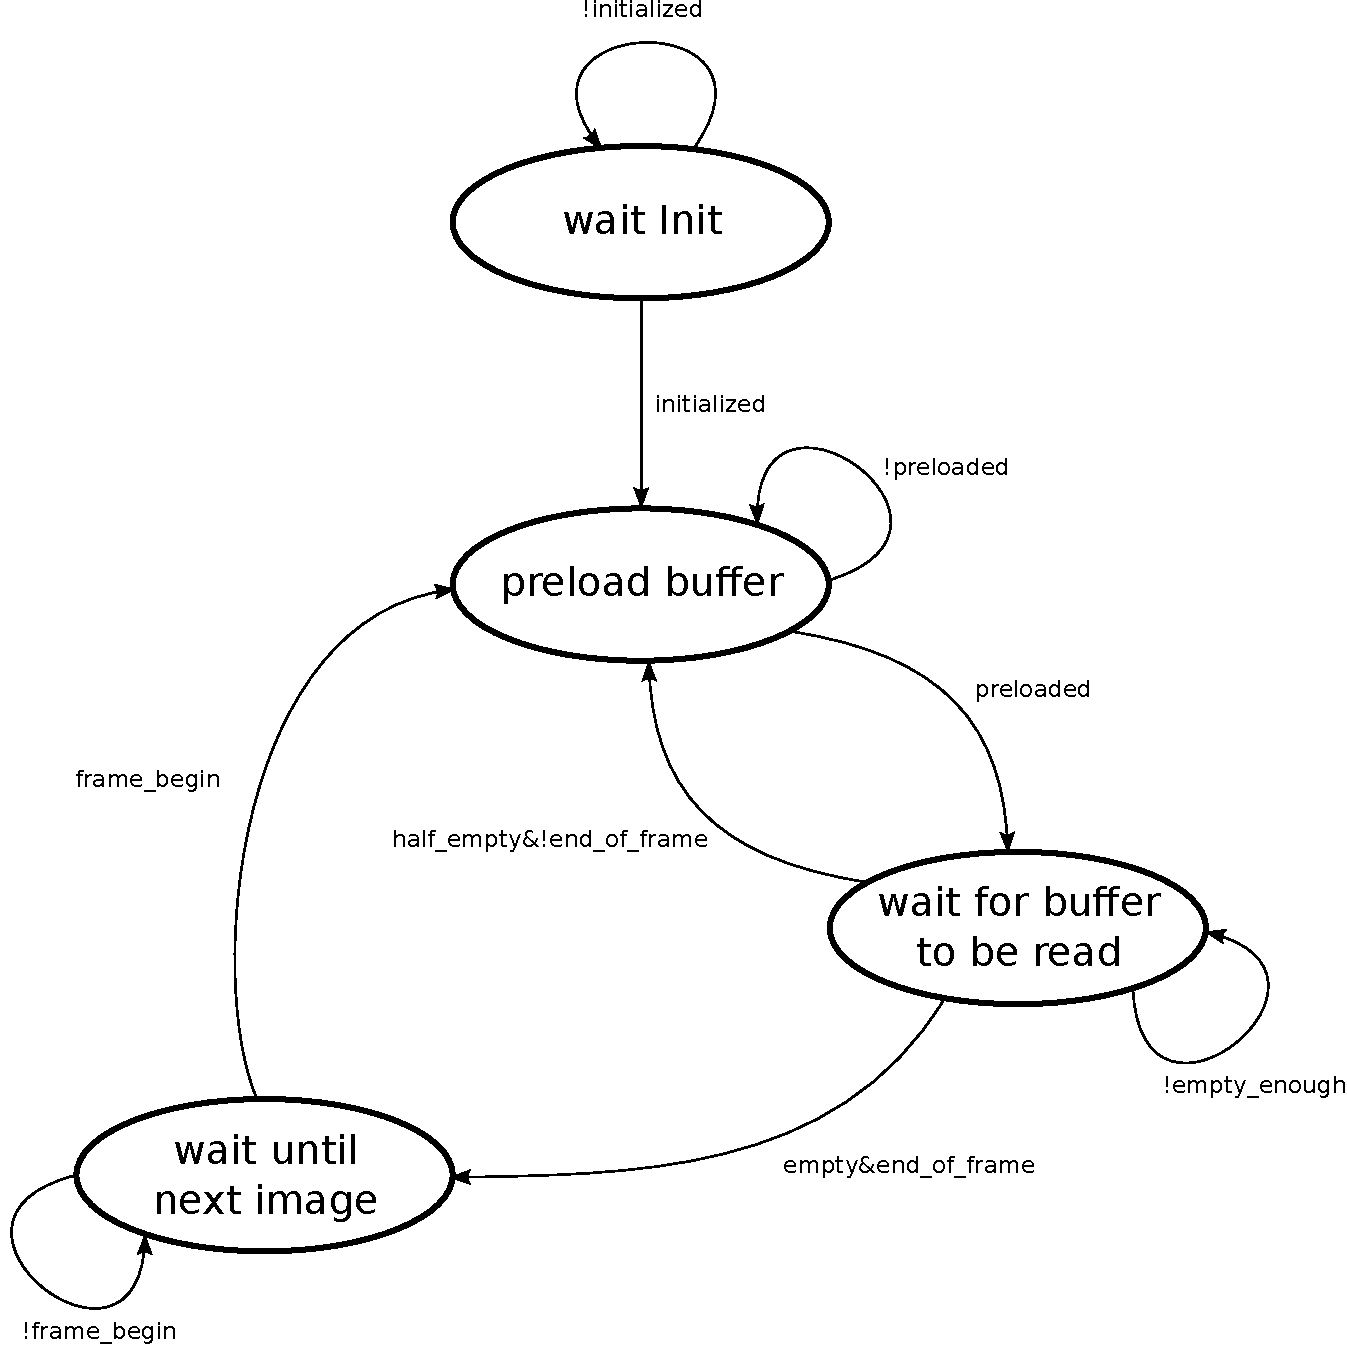
\includegraphics[width=11cm]{figs/video_out_sm.pdf}
\caption{VideoOut's behavior}
\label{VideoOut_behavior}
\end{figure}

